%************************************************
\chapter{Causal Hypotheses}
\label{chapter:causal_hypotheses}
%************************************************

\section{Representing Static Space}

Spatial arrangements of static symbols are created by the reflective
thinking layers.  Static symbols are not contained within the physical
layer, but these symbols are used to represent transitions from the
past to the future, which are in turn used to create relationships
between causes and effects that are used for planning.  Thinking
activities use these Spatial arrangements of symbols to think about
the given activities of the physical layer as well as planning in the
first-order reflective layer.

\section{Representing Simultaneities}

\begin{figure}
\center
\includegraphics[width=10cm]{gfx}/example_simultaneity
\caption{Example simultaneity.}
\label{figure:example_simultaneity}
\end{figure}

\section{Representing Transitions}

As {\mbox{\autoref{equation:define_symbol_referent_graph}}} states,
each reflective thinking layer can create symbolic references to
dynamic activities in the layers below as well as any other symbolic
activities in or below the symbolization activity.  Simultaneities and
transitions are the basis for representing concurrent and sequential
event knowledge.  It is a type of static Spatial arrangement between
static symbolic references.  Simultaneities and transitions can be
arranged into sequences back in time, forward in time, as well as
organizing time into binary trees for efficient recall.
\begin{figure}
\center
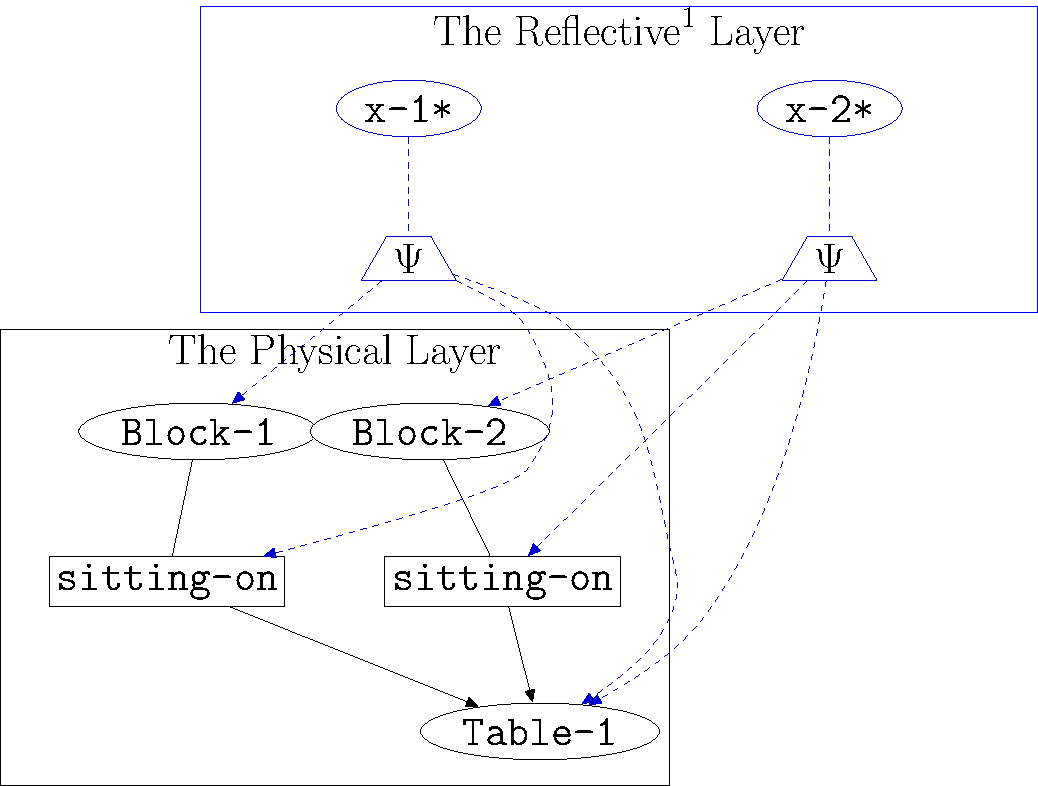
\includegraphics[width=10cm]{gfx/two_example_grounded_symbolic_references}
\caption[Two example symbolic references.]{Two example grounded
  symbolic references, $x_1^*$ and $x_2^*$.}
\label{figure:two_example_grounded_symbolic_references}
\end{figure}
\begin{figure}
\center
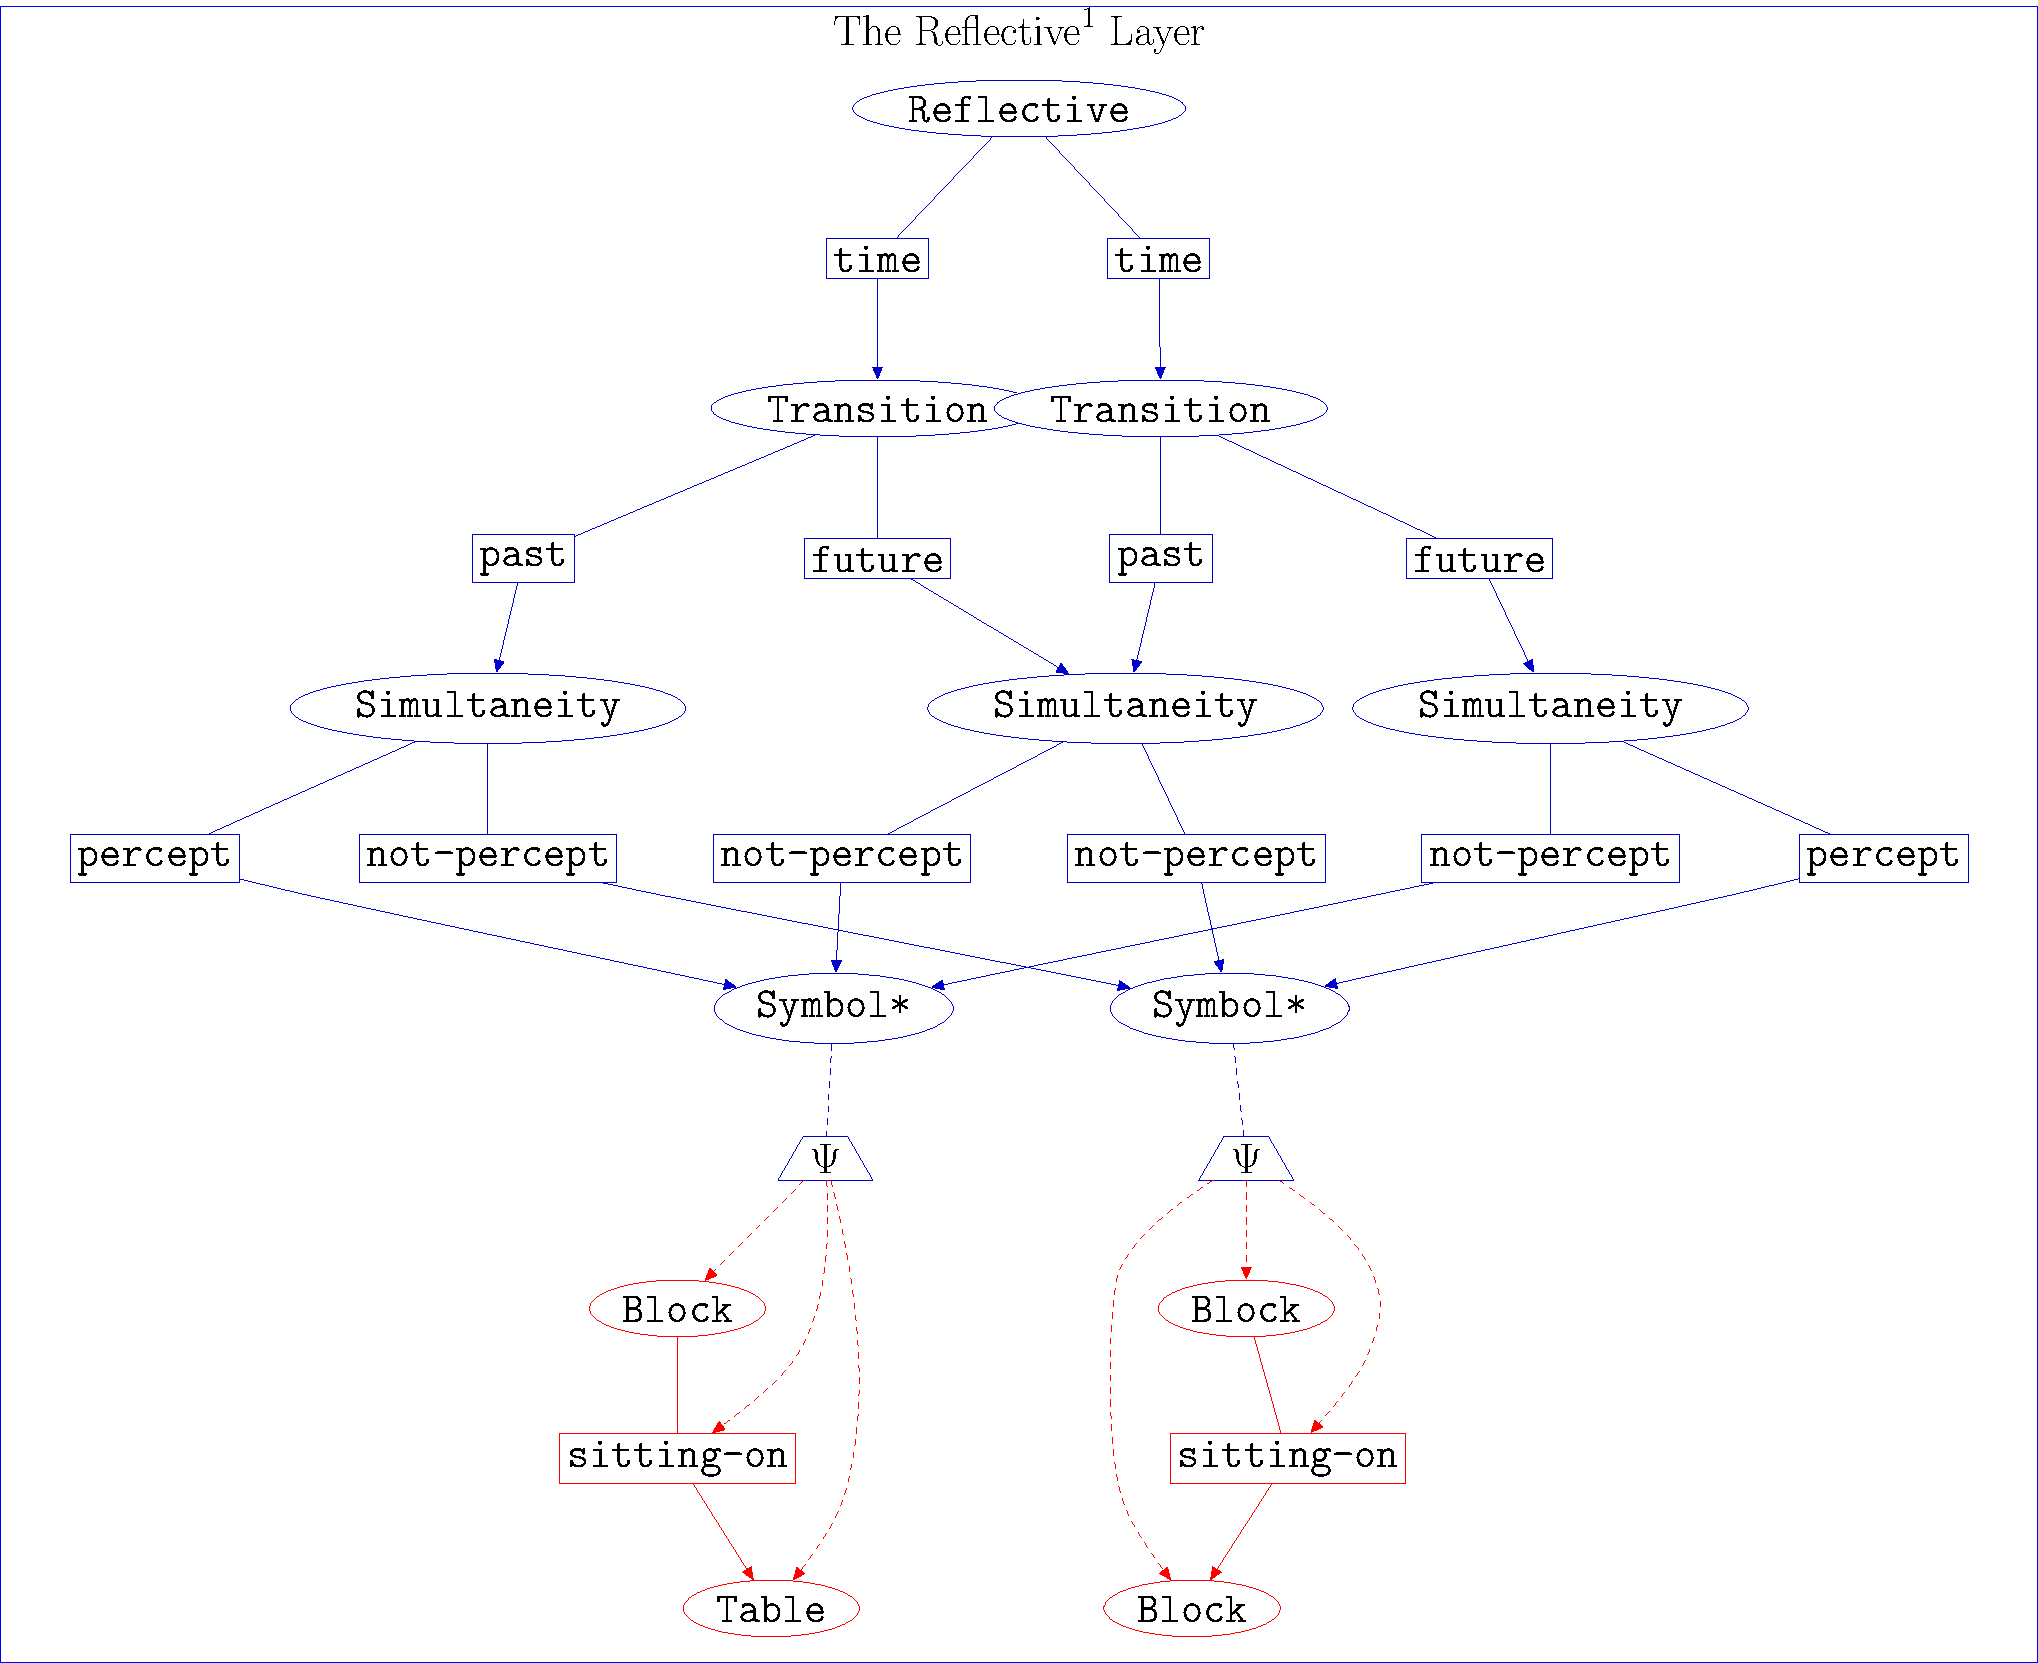
\includegraphics[width=10cm]{gfx/example_transition}
\caption[An example of a transition between simultaneities.]{An
  example of a transition between simultaneities, $t_1^*$ and $t_2^*$,
  of first-order static symbolic references, $x_1^*$ and $x_2^*$.}
\label{figure:example_transition}
\end{figure}

\section{Representing Causal Hypotheses}

\begin{figure}
\center
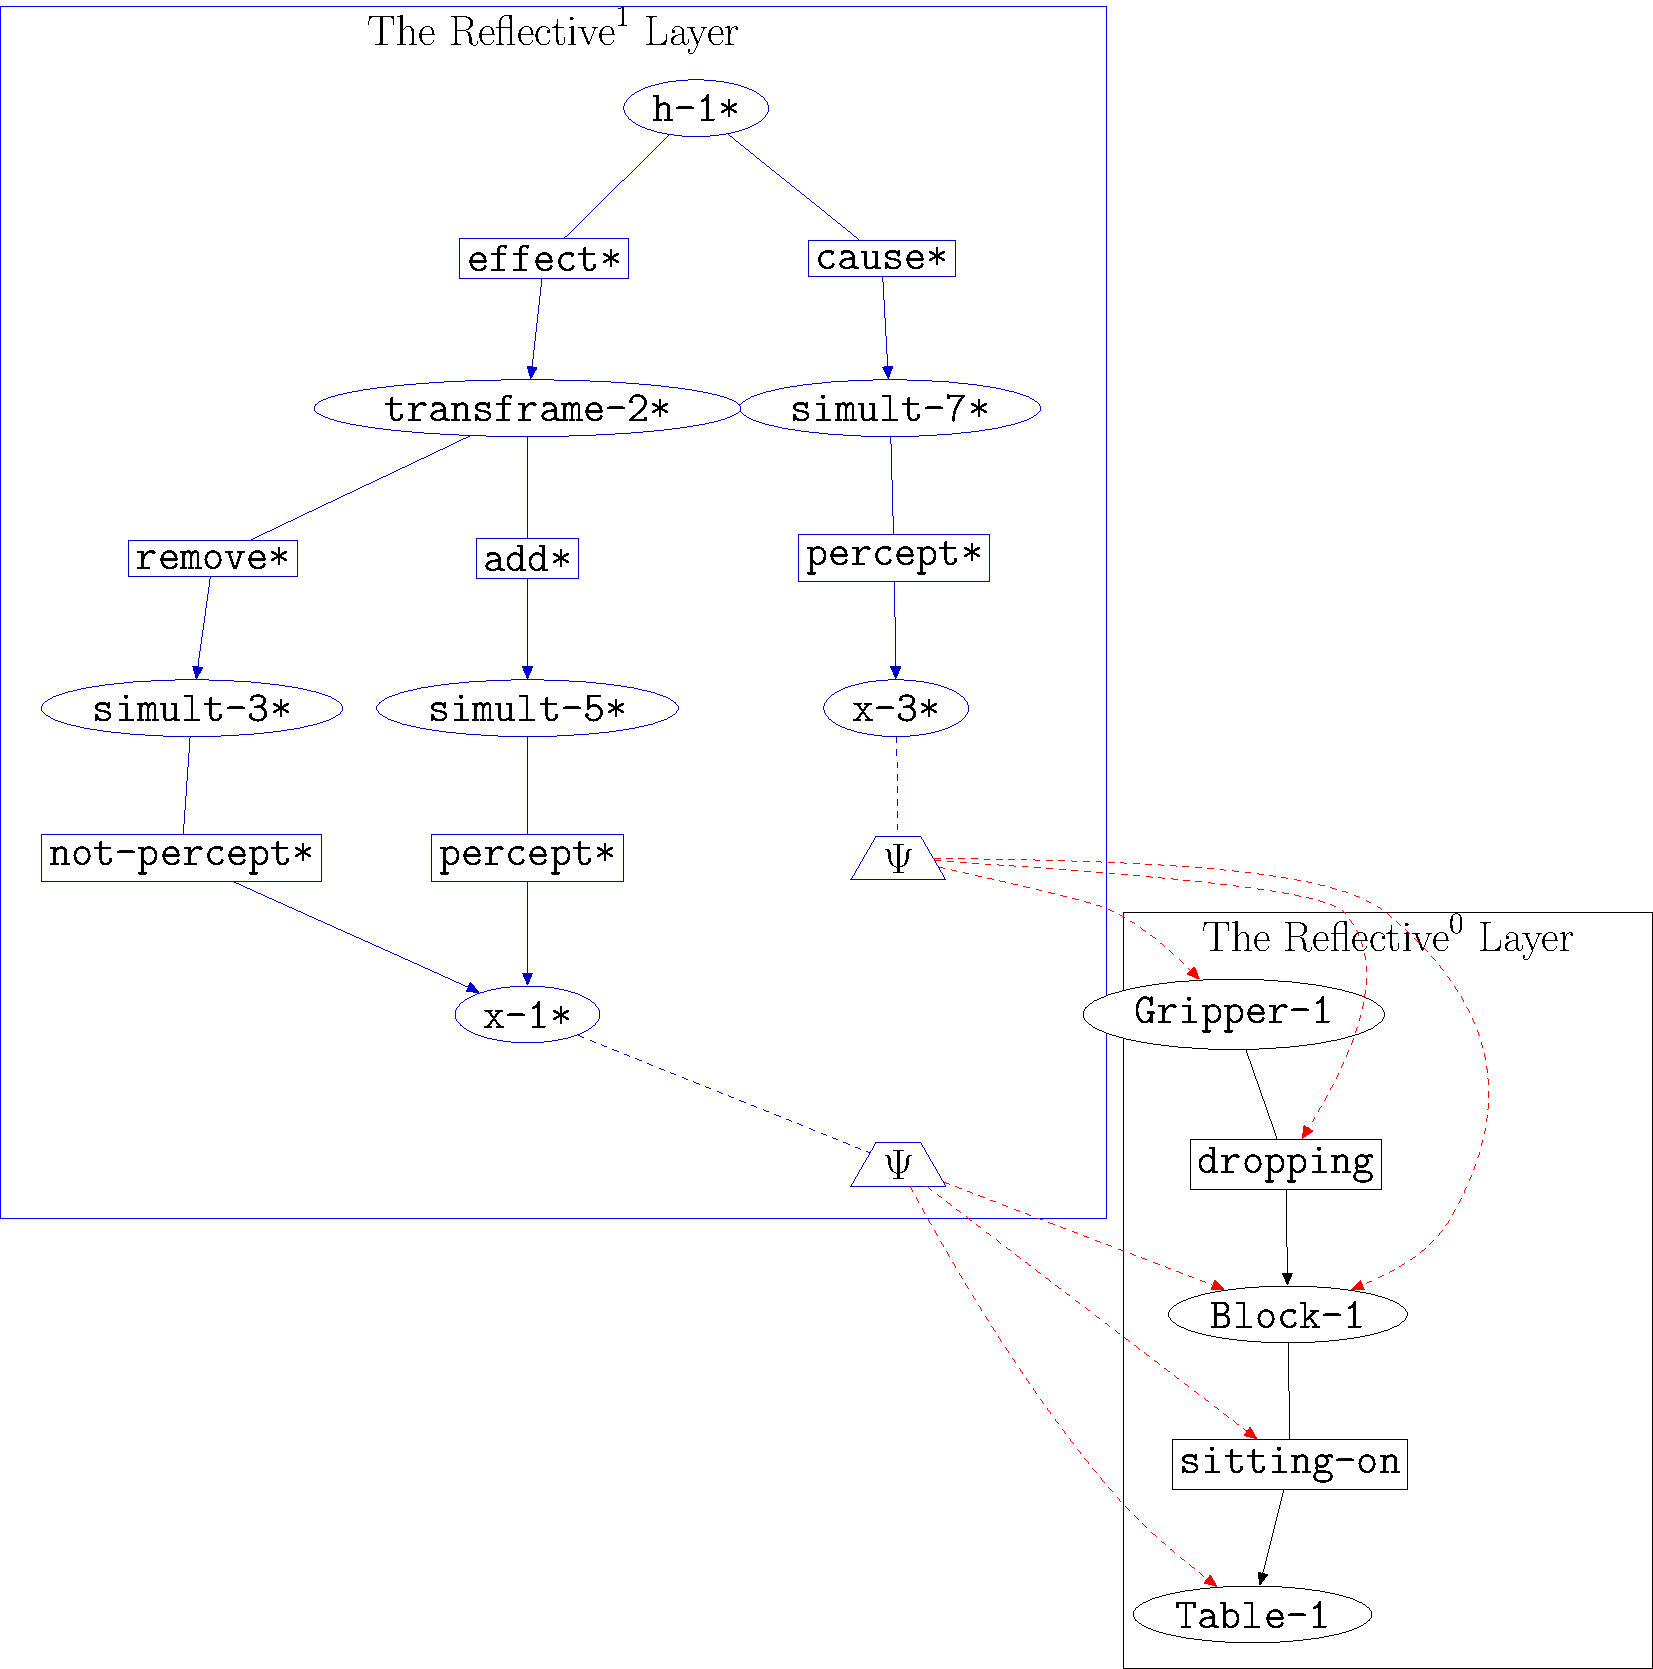
\includegraphics[width=10cm]{gfx/example_causal_hypothesis}
\caption{An example of a causal hypothesis.}
\label{figure:example_causal_hypothesis}
\end{figure}

